\hypertarget{markov-chain-monte-carlo}{%
\section{Markov Chain Monte Carlo}\label{markov-chain-monte-carlo}}

Markov Chain Monte Carlo (MCMC) is a useful method whenever we have a probability distribution that we want to sample from but there is not direct sampling way to do so.

\hypertarget{direct-random-sampling}{%
\subsection{Direct Random Sampling}\label{direct-random-sampling}}

In almost any computer simulation the ultimate source of randomness is a stream of (close to) uniform, uncorrelated bits generated from a pseudo random number generator. A direct sampling method takes such a source and outputs uncorrelated samples from the target distribution. The fact they're uncorrelated is key as we'll see later. Examples of direct sampling methods range from the trivial: take n random bits to generate integers uniformly between 0 and \(2^n\) to more complex methods such as inverse transform sampling and rejection sampling~\autocite{devroyeRandomSampling1986}.

In physics the distribution we usually want to sample from is the Boltzmann probability over states of the system \(S\): \[
\begin{aligned}
p(S)  &= \frac{1}{\mathcal{Z}} e^{-\beta H(S)} \\
\end{aligned}
\] where \(\mathcal{Z} = \sum_S e^{-\beta H(S)}\) is the normalisation factor and ubiquitous partition function. In principle we could directly sample from this, for a discrete system there are finitely many choices. We could calculate the probability of each one and assign each a region of the unit interval which we could then sample uniformly from.

However if we actually try to do this we will run into two problems, we can't calculate \(\mathcal{Z}\) for any reasonably sized systems because the state space grows exponentially with system size. Even if we could calculate \(\mathcal{Z}\), sampling from an exponentially large number of options quickly become tricky. This kind of problem happens in many other disciplines too, particularly when fitting statistical models using Bayesian inference~\autocite{BMCP2021}.

\hypertarget{mcmc-sampling}{%
\subsection{MCMC Sampling}\label{mcmc-sampling}}

So what can we do? Well it turns out that if we're willing to give up in the requirement that the samples be uncorrelated then we can use MCMC instead.

MCMC defines a weighted random walk over the states \((S_0, S_1, S_2, ...)\), such that in the long time limit, states are visited according to their probability \(p(S)\).~\autocite{binderGuidePracticalWork1988,kerteszAdvancesComputerSimulation1998,wolffMonteCarloErrors2004}. ~\autocite{krauthIntroductionMonteCarlo1998}

\[\lim_{i\to\infty} p(S_i) = P(S)\]

In a physics context this lets us evaluate any observable with a mean over the states visited by the walk. \[\begin{aligned}
\langle O \rangle & = \sum_{S} p(S) \langle O \rangle_{S} = \sum_{i = 0}^{M} \langle O\rangle_{S_i} + \mathcal{O}(\tfrac{1}{\sqrt{M}})\\
\end{aligned}\]

The the samples in the random walk are correlated so the samples effectively contain less information than \(N\) independent samples would. As a consequence the variance is larger than the \(\langle O^2 \rangle - \langle O\rangle^2\) form it would have if the estimates were uncorrelated. Methods of estimating the true variance of \(\langle O \rangle\) and decided how many steps are needed will be considered later.

\hypertarget{implementation-of-mcmc}{%
\subsection{Implementation of MCMC}\label{implementation-of-mcmc}}

In implementation MCMC can be boiled down to choosing a transition function \$\mathcal{T}(S\_\{t\} \rightarrow S\_\{t+1\}) \$ where \(S\) are vectors representing classical spin configurations. We start in some initial state \(S_0\) and then repeatedly jump to new states according to the probabilities given by \(\mathcal{T}\). This defines a set of random walks \(\{S_0\ldots S_i\ldots S_N\}\).

In pseudo-code one could write the MCMC simulation for a single walker as:

\begin{Shaded}
\begin{Highlighting}[]
\NormalTok{current\_state }\OperatorTok{=}\NormalTok{ initial\_state}

\ControlFlowTok{for}\NormalTok{ i }\KeywordTok{in} \BuiltInTok{range}\NormalTok{(N\_steps):}
\NormalTok{    new\_state }\OperatorTok{=}\NormalTok{ sample\_T(current\_state) }
\NormalTok{    states[i] }\OperatorTok{=}\NormalTok{ current\_state}
\end{Highlighting}
\end{Shaded}

Where the \texttt{sample\_T} function samples directly from the transition function \(\mathcal{T}\).

If we run many such walkers in parallel we can then approximate the distribution \(p_t(S; S)\) which tells us where the walkers are likely to be after they've evolved for \(t\) steps from an initial state \(S_0\). We need to carefully choose \(\mathcal{T}\) such that the the probability \(p_t(S; S_0)\) approaches the distribution of interest. In this case the thermal distribution \(P(S; \beta) = \mathcal{Z}^{-1} e^{-\beta F(S)}\).

\hypertarget{global-and-detailed-balance-equations}{%
\subsection{Global and Detailed balance equations}\label{global-and-detailed-balance-equations}}

We cam quite easily write down the properties that \(\mathcal{T}\) must have in order to yield the correct target distribution. Since we must transition somewhere at each step, we first have the normalisation condition that \[\sum\limits_S \mathcal{T}(S' \rightarrow S) = 1.\]

Second, let us move to an ensemble view, where rather than individual walkers and states, we think about the probability distribution of many walkers at each step. If we start all the walkers in the same place the initial distribution will be a delta function and as we step the walkers will wander around, giving us a sequence of probability distributions \(\{p_0(S), p_1(S), p_2(S)\ldots\}\). For discrete spaces we can write the action of the transition function on \(p_i\) as a matrix equation

\[\begin{aligned}
p_{i+1}(S) &= \sum_{S' \in \{S\}} p_i(S') \mathcal{T}(S' \rightarrow S)
\end{aligned}\]

This equation is essentially just stating that total probability mass is conserved as our walkers flow around the state space.

In order that \(p_i\) converges to our target distribution \(p\) in the long time limit, we need the target distribution to be a fixed point of the transition function

\[\begin{aligned}
P(S) &= \sum_{S'} P(S') \mathcal{T}(S' \rightarrow S)
\end{aligned}
\] Along with some more technical considerations such as ergodicity which won't be considered here, global balance suffices to ensure that a MCMC method is correct~\autocite{kellyReversibilityStochasticNetworks1981}.

A sufficient but not necessary condition for global balance to hold is called detailed balance:

\[
P(S) \mathcal{T}(S \rightarrow S') = P(S') \mathcal{T}(S' \rightarrow S)
\]

In practice most algorithms are constructed to satisfy detailed rather than global balance, though there are arguments that the relaxed requirements of global balance can lead to faster algorithms~\autocite{kapferSamplingPolytopeHarddisk2013}.

The goal of MCMC is then to choose \(\mathcal{T}\) so that it has the desired thermal distribution \(P(S)\) as its fixed point and converges quickly onto it. This boils down to requiring that the matrix representation of \(T_{ij} = \mathcal{T}(S_i \to S_j)\) has an eigenvector with entries \(P_i = P(S_i)\) with eigenvalue 1 and all other eigenvalues with magnitude less than one. The convergence time depends on the magnitude of the second largest eigenvalue.

The choice of the transition function for MCMC is under-determined as one only needs to satisfy a set of balance conditions for which there are many solutions~\autocite{kellyReversibilityStochasticNetworks1981}. The standard choice that satisfies these requirements is called the Metropolis-Hastings algorithm.

\hypertarget{the-metropolis-hastings-algorithm}{%
\subsection{The Metropolis-Hastings Algorithm}\label{the-metropolis-hastings-algorithm}}

The Metropolis-Hastings algorithm breaks the transition function into a proposal distribution \(q(S \to S')\) and an acceptance function \(\mathcal{A}(S \to S')\). \(q\) must be a function we can directly sample from, and in many cases takes the form of flipping some number of spins in \(S\), i.e if we're flipping a single random spin in the spin chain, \(q(S \to S')\) is the uniform distribution on states reachable by one spin flip from \(S\). This also gives the symmetry property that \(q(S \to S') = q(S' \to S)\).

The proposal \(S'\) is then accepted or rejected with an acceptance probability \(\mathcal{A}(S \to S')\), if the proposal is rejected then \(S_{i+1} = S_{i}\). Hence:

\[\mathcal{T}(S\to S') = q(S\to S')\mathcal{A}(S \to S')\]

The Metropolis-Hasting algorithm is a slight extension of the original Metropolis algorithm which allows for non-symmetric proposal distributions \$q(S\to S') \neq q(S'\to S) \$. It can be derived starting from detailed balance~\autocite{krauthIntroductionMonteCarlo1998}:

\[
P(S)\mathcal{T}(S \to S') = P(S')\mathcal{T}(S' \to S)
\]

inserting the proposal and acceptance function

\[
P(S)q(S \to S')\mathcal{A}(S \to S') = P(S')q(S' \to S)\mathcal{A}(S' \to S)
\]

rearranging gives us a condition on the acceptance function in terms of the target distribution and the proposal distribution which can be thought of as inputs to the algorithm

\[
\frac{\mathcal{A}(S \to S')}{\mathcal{A}(S' \to S)} = \frac{P(S')q(S' \to S)}{P(S)q(S \to S')} = f(S, S')
\]

The Metropolis-Hastings algorithm is the choice

\[
\begin{aligned}
\label{eq:mh} 
\mathcal{A}(S \to S') = \min\left(1, f(S,S')\right)
\end{aligned}
\] for the acceptance function. The proposal distribution is left as a free choice.

Noting that \(f(S,S') = 1/f(S',S)\), we can see that the MH algorithm satifies detailed balance by considering the two cases \(f(S,S') > 1\) and \(f(S,S') < 1\).

By choosing the proposal distribution such that \(f(S,S')\) is as close as possible to one, the rate of rejections can be reduced and the algorithm sped up. This can be challenging though, as getting \(f(S,S')\) close to 1 would imply that we can directly sample from a distribution very close to the target distribution. As MCMC is usually applied to problems for which there is virtually no hope of sampling directly from the target distribution, it's rare that one can do so approximately.

When the proposal distribution is symmetric as ours is, it cancels out in the expression for the acceptance function and the Metropolis-Hastings algorithm is simply the choice

\[\mathcal{A}(S \to S') = \min\left(1, e^{-\beta\;\Delta F}\right)\]

where \(F\) is the overall free energy of the system, including both the quantum and classical sector.

\hypertarget{implementation-of-the-mh-algorithm}{%
\subsection{Implementation of the MH Algorithm}\label{implementation-of-the-mh-algorithm}}

To implement the acceptance function in practice we pick a random number in the unit interval and accept if it is less than \(e^{-\beta\;\Delta F}\):

\begin{Shaded}
\begin{Highlighting}[]
\NormalTok{current\_state }\OperatorTok{=}\NormalTok{ initial\_state}

\ControlFlowTok{for}\NormalTok{ i }\KeywordTok{in} \BuiltInTok{range}\NormalTok{(N\_steps):}
\NormalTok{    new\_state }\OperatorTok{=}\NormalTok{ proposal(current\_state)}
\NormalTok{    df }\OperatorTok{=}\NormalTok{ free\_energy\_change(current\_state, new\_state, parameters)}

    \ControlFlowTok{if}\NormalTok{ uniform(}\DecValTok{0}\NormalTok{,}\DecValTok{1}\NormalTok{) }\OperatorTok{\textless{}}\NormalTok{ exp(}\OperatorTok{{-}}\NormalTok{beta }\OperatorTok{*}\NormalTok{ df):}
\NormalTok{        current\_state }\OperatorTok{=}\NormalTok{ new\_state}
        
\NormalTok{    states[i] }\OperatorTok{=}\NormalTok{ current\_state}
\end{Highlighting}
\end{Shaded}

\hypertarget{the-metropolis-hasting-algorithm}{%
\subsection{The Metropolis-Hasting Algorithm}\label{the-metropolis-hasting-algorithm}}

\hypertarget{metropolis-hastings}{%
\subsection{Metropolis-Hastings}\label{metropolis-hastings}}

In order to actually choose new states according to \(\mathcal{T}\) one chooses states from a proposal distribution \(q(S_i \to S')\) that can be directly sampled from. For instance, this might mean flipping a single random spin in a spin chain, in which case \(q(x_i\to x_i)\) is the uniform distribution on states reachable by one spin flip from \(x_i\). The proposal \(S'\) is then accepted or rejected with an acceptance probability \(\mathcal{A}(x_i\to x_{i+1})\), if the proposal is rejected then \(x_{i+1} = x_{i}\). Now \(\mathcal{T}(S\to S') = q(S\to S')\mathcal{A}(S \to S')\).

\hypertarget{the-metropolis-hastings-algorithm-1}{%
\subsubsection{The Metropolis-Hastings Algorithm}\label{the-metropolis-hastings-algorithm-1}}

MH breaks up the transition function into a proposal distribution \(q(S \to S')\) and an acceptance function \(\mathcal{A}(S \to S')\). \(q\) needs to be something that we can directly sample from, and in our case generally takes the form of flipping some number of spins in \(S\), i.e if we're flipping a single random spin in the spin chain, \(q(S \to S')\) is the uniform distribution on states reachable by one spin flip from \(S\). This also gives the nice symmetry property that \(q(S \to S') = q(S' \to S)\).

The proposal \(S'\) is then accepted or rejected with an acceptance probability \(\mathcal{A}(S \to S')\), if the proposal is rejected then \(S_{i+1} = S_{i}\). Hence:

\[\mathcal{T}(S\to S') = q(S\to S')\mathcal{A}(S \to S')\]

When the proposal distribution is symmetric as ours is, it cancels out in the expression for the acceptance function and the Metropolis-Hastings algorithm is simply the choice: \[ \mathcal{A}(S \to S') = \min\left(1, e^{-\beta\;\Delta F}\right)\] Where \(F\) is the overall free energy of the system, including both the quantum and classical sector.

To implement the acceptance function in practice we pick a random number in the unit interval and accept if it is less than \(e^{-\beta\;\Delta F}\):

\begin{Shaded}
\begin{Highlighting}[]
\NormalTok{current\_state }\OperatorTok{=}\NormalTok{ initial\_state}

\ControlFlowTok{for}\NormalTok{ i }\KeywordTok{in} \BuiltInTok{range}\NormalTok{(N\_steps):}
\NormalTok{    new\_state }\OperatorTok{=}\NormalTok{ proposal(current\_state)}
\NormalTok{    df }\OperatorTok{=}\NormalTok{ free\_energy\_change(current\_state, new\_state, parameters)}

    \ControlFlowTok{if}\NormalTok{ uniform(}\DecValTok{0}\NormalTok{,}\DecValTok{1}\NormalTok{) }\OperatorTok{\textless{}}\NormalTok{ exp(}\OperatorTok{{-}}\NormalTok{beta }\OperatorTok{*}\NormalTok{ df):}
\NormalTok{        current\_state }\OperatorTok{=}\NormalTok{ new\_state}
        
\NormalTok{    states[i] }\OperatorTok{=}\NormalTok{ current\_state}
\end{Highlighting}
\end{Shaded}

This has the effect of always accepting proposed states that are lower in energy and sometimes accepting those that are higher in energy than the current state.

\hypertarget{two-step-trick}{%
\subsection{Two Step Trick}\label{two-step-trick}}

Our method already relies heavily on the split between the classical and quantum sector to derive a sign problem free MCMC algorithm but it turns out that there is a further trick we can play with it. The free energy term is the sum of an easy to compute classical energy and a more expensive quantum free energy, we can split the acceptance function into two in such as way as to avoid having to compute the full exact diagonalisation some of the time:

\begin{Shaded}
\begin{Highlighting}[]
\NormalTok{current\_state }\OperatorTok{=}\NormalTok{ initial\_state}

\ControlFlowTok{for}\NormalTok{ i }\KeywordTok{in} \BuiltInTok{range}\NormalTok{(N\_steps):}
\NormalTok{    new\_state }\OperatorTok{=}\NormalTok{ proposal(current\_state)}

\NormalTok{    df\_classical }\OperatorTok{=}\NormalTok{ classical\_free\_energy\_change(current\_state, new\_state, parameters)}
    \ControlFlowTok{if}\NormalTok{ exp(}\OperatorTok{{-}}\NormalTok{beta }\OperatorTok{*}\NormalTok{ df\_classical) }\OperatorTok{\textless{}}\NormalTok{ uniform(}\DecValTok{0}\NormalTok{,}\DecValTok{1}\NormalTok{):}
\NormalTok{        f\_quantum }\OperatorTok{=}\NormalTok{ quantum\_free\_energy(current\_state, new\_state, parameters)}
    
        \ControlFlowTok{if}\NormalTok{ exp(}\OperatorTok{{-}}\NormalTok{ beta }\OperatorTok{*}\NormalTok{ df\_quantum) }\OperatorTok{\textless{}}\NormalTok{ uniform(}\DecValTok{0}\NormalTok{,}\DecValTok{1}\NormalTok{):}
\NormalTok{          current\_state }\OperatorTok{=}\NormalTok{ new\_state}
    
\NormalTok{        states[i] }\OperatorTok{=}\NormalTok{ current\_state}
    
\end{Highlighting}
\end{Shaded}

\hypertarget{detailed-balance-for-the-two-step-method}{%
\subsection{Detailed Balance for the two step method}\label{detailed-balance-for-the-two-step-method}}

Given a MCMC algorithm with target distribution \(\pi(a)\) and transition function \(\mathcal{T}\) the detailed balance condition is sufficient (along with some technical constraints~\autocite{wolffMonteCarloErrors2004}) to guarantee that in the long time limit the algorithm produces samples from \(\pi\). \[\pi(a)\mathcal{T}(a \to b) = \pi(b)\mathcal{T}(b \to a)\]

In pseudo-code, our two step method corresponds to two nested comparisons with the majority of the work only occurring if the first test passes:

\begin{Shaded}
\begin{Highlighting}[]
\NormalTok{current\_state }\OperatorTok{=}\NormalTok{ initial\_state}

\ControlFlowTok{for}\NormalTok{ i }\KeywordTok{in} \BuiltInTok{range}\NormalTok{(N\_steps):}
\NormalTok{  new\_state }\OperatorTok{=}\NormalTok{ proposal(current\_state)}

\NormalTok{  c\_dE }\OperatorTok{=}\NormalTok{ classical\_energy\_change(}
\NormalTok{                               current\_state,}
\NormalTok{                               new\_state)}
  \ControlFlowTok{if}\NormalTok{ uniform(}\DecValTok{0}\NormalTok{,}\DecValTok{1}\NormalTok{) }\OperatorTok{\textless{}}\NormalTok{ exp(}\OperatorTok{{-}}\NormalTok{beta }\OperatorTok{*}\NormalTok{ c\_dE):}
\NormalTok{    q\_dF }\OperatorTok{=}\NormalTok{ quantum\_free\_energy\_change(}
\NormalTok{                                current\_state,}
\NormalTok{                                new\_state)}
    \ControlFlowTok{if}\NormalTok{ uniform(}\DecValTok{0}\NormalTok{,}\DecValTok{1}\NormalTok{) }\OperatorTok{\textless{}}\NormalTok{ exp(}\OperatorTok{{-}}\NormalTok{ beta }\OperatorTok{*}\NormalTok{ q\_dF):}
\NormalTok{      current\_state }\OperatorTok{=}\NormalTok{ new\_state}

\NormalTok{    states[i] }\OperatorTok{=}\NormalTok{ current\_state}
\end{Highlighting}
\end{Shaded}

Defining \(r_c = e^{-\beta H_c}\) and \(r_q = e^{-\beta F_q}\) our target distribution is \(\pi(a) = r_c r_q\). This method has \(\mathcal{T}(a\to b) = q(a\to b)\mathcal{A}(a \to b)\) with symmetric \(p(a \to b) = \pi(b \to a)\) and \(\mathcal{A} = \min\left(1, r_c\right) \min\left(1, r_q\right)\)

Substituting this into the detailed balance equation gives: \[\mathcal{T}(a \to b)/\mathcal{T}(b \to a) = \pi(b)/\pi(a) = r_c r_q\]

Taking the LHS and substituting in our transition function: \[\begin{aligned}
\mathcal{T}(a \to b)/\mathcal{T}(b \to a) = \frac{\min\left(1, r_c\right) \min\left(1, r_q\right)}{ \min\left(1, 1/r_c\right) \min\left(1, 1/r_q\right)}\end{aligned}\]

which simplifies to \(r_c r_q\) as \(\min(1,r)/\min(1,1/r) = r\) for \(r > 0\).

\hypertarget{two-step-trick-1}{%
\subsubsection{Two Step Trick}\label{two-step-trick-1}}

Our method already relies heavily on the split between the classical and quantum sector to derive a sign problem free MCMC algorithm but it turns out that there is a further trick we can play with it. The free energy term is the sum of an easy to compute classical energy and a more expensive quantum free energy, we can split the acceptance function into two in such as way as to avoid having to compute the full exact diagonalisation some of the time:

\begin{Shaded}
\begin{Highlighting}[]

\NormalTok{current\_state }\OperatorTok{=}\NormalTok{ initial\_state}

\ControlFlowTok{for}\NormalTok{ i }\KeywordTok{in} \BuiltInTok{range}\NormalTok{(N\_steps):}
\NormalTok{    new\_state }\OperatorTok{=}\NormalTok{ proposal(current\_state)}

\NormalTok{    df\_classical }\OperatorTok{=}\NormalTok{ classical\_free\_energy\_change(current\_state, new\_state, parameters)}
    \ControlFlowTok{if}\NormalTok{ exp(}\OperatorTok{{-}}\NormalTok{beta }\OperatorTok{*}\NormalTok{ df\_classical) }\OperatorTok{\textless{}}\NormalTok{ uniform(}\DecValTok{0}\NormalTok{,}\DecValTok{1}\NormalTok{):}
\NormalTok{        f\_quantum }\OperatorTok{=}\NormalTok{ quantum\_free\_energy(current\_state, new\_state, parameters)}
    
        \ControlFlowTok{if}\NormalTok{ exp(}\OperatorTok{{-}}\NormalTok{ beta }\OperatorTok{*}\NormalTok{ df\_quantum) }\OperatorTok{\textless{}}\NormalTok{ uniform(}\DecValTok{0}\NormalTok{,}\DecValTok{1}\NormalTok{):}
\NormalTok{          current\_state }\OperatorTok{=}\NormalTok{ new\_state}
    
\NormalTok{        states[i] }\OperatorTok{=}\NormalTok{ current\_state}
    
\end{Highlighting}
\end{Shaded}

\hypertarget{auto-correlation-time}{%
\subsubsection{Auto-correlation Time}\label{auto-correlation-time}}

\hypertarget{fig:m_autocorr}{%
\begin{figure}
\centering
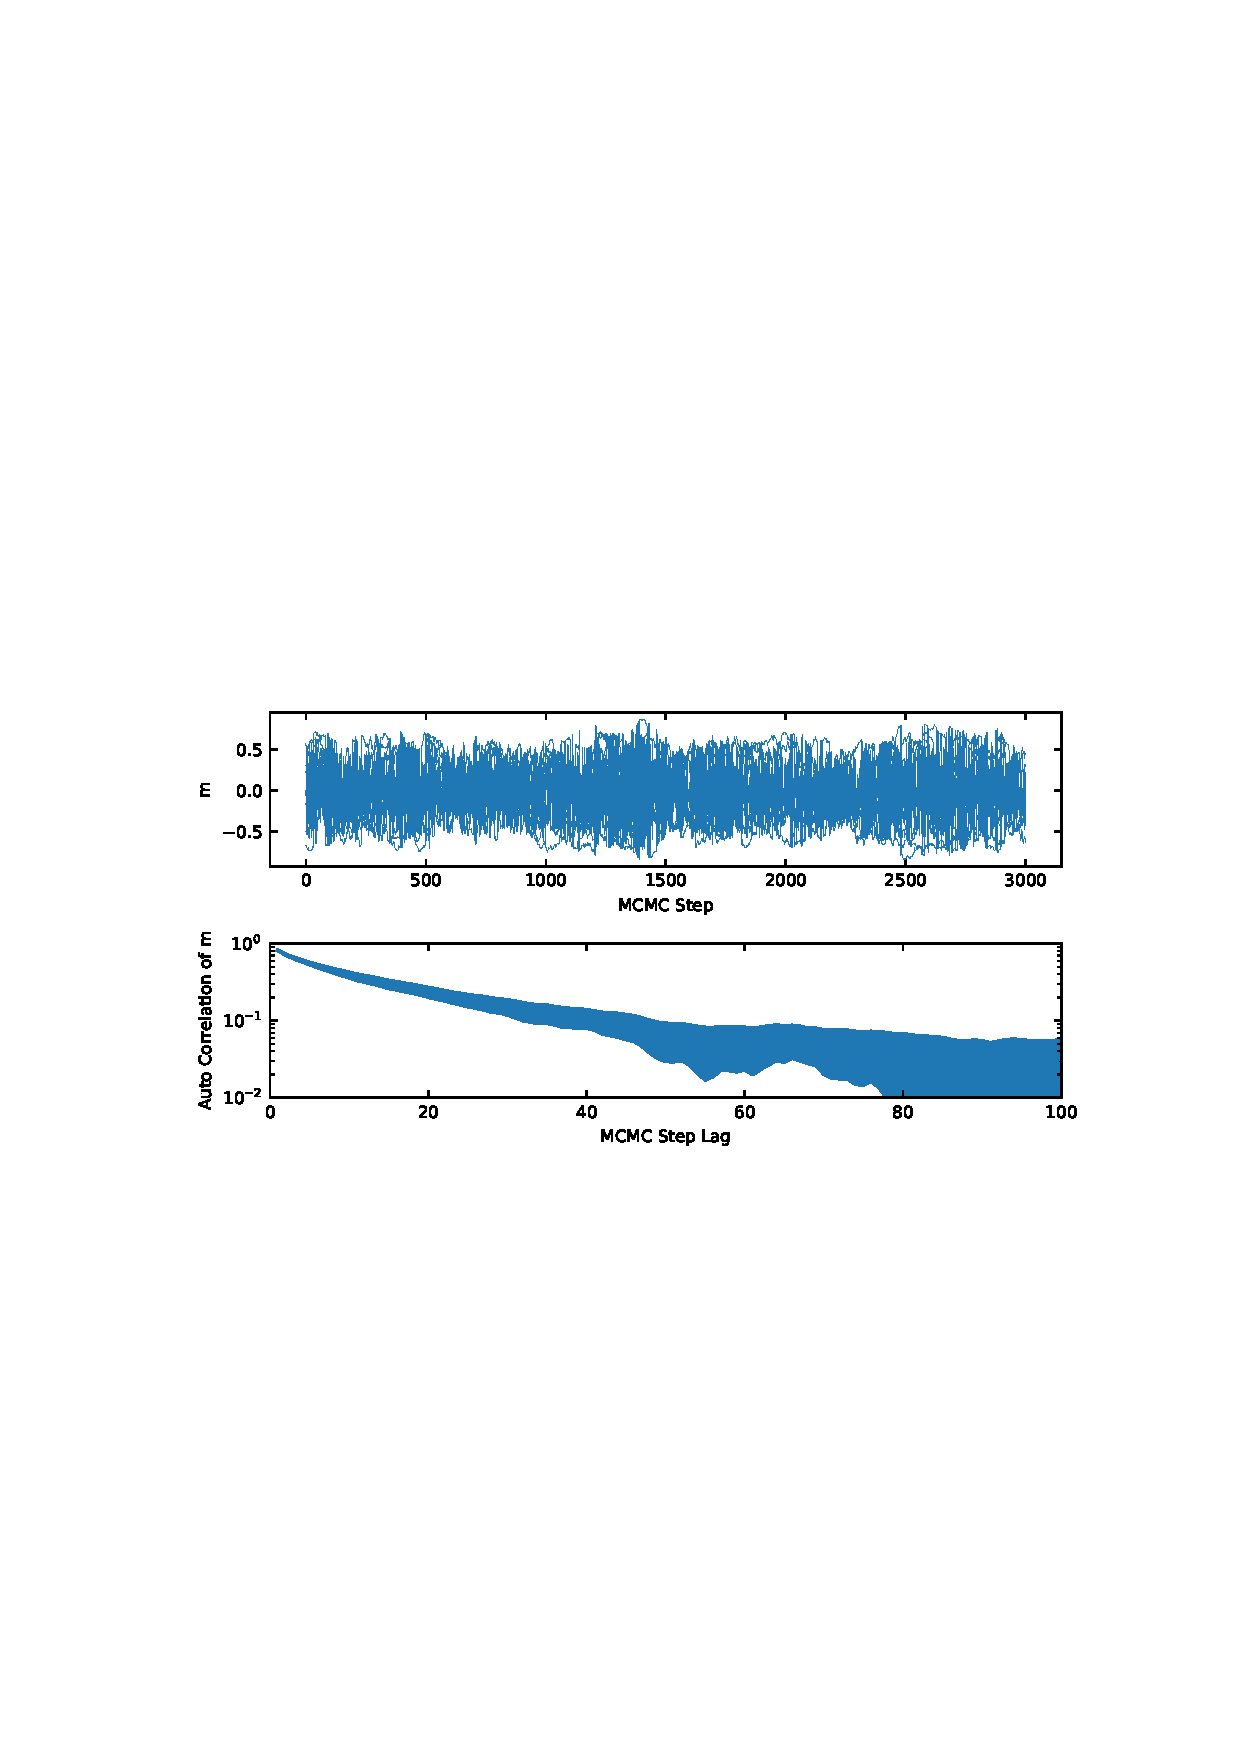
\includegraphics[width=1\textwidth,height=\textheight]{figure_code/fk_chapter/lsr/figs/m_autocorr.png}
\caption[{no title}]{(Upper) 10 MCMC chains starting from the same initial state for a system with \(N = 150\) sites and 3000 MCMC steps. At each MCMC step, n spins are flipped where n is drawn from Uniform(1,N) and this is repeated \(N^2/100\) times. The simulations therefore have the potential to necessitate \(10*N^2\) matrix diagonalisations for each 100 MCMC steps. (Lower) The normalised auto-correlation \((\langle m_i m_{i-j}\rangle - \langle m_i\rangle \langle m_i \rangle) / Var(m_i))\) averaged over \(i\). It can be seen that even with each MCMC step already being composed of many individual flip attempts, the auto-correlation is still non negligible and must be taken into account in the statistics. \(t = 1, \alpha = 1.25, T = 2.2, J = U = 5\)}
\label{fig:m_autocorr}
\end{figure}
}

At this stage one might think we're done. We can indeed draw independent samples from \(P(S; \beta)\) by starting from some arbitrary initial state and doing \(k\) steps to arrive at a sample. However a key insight is that after the convergence time, every state generated is a sample from \(P(S; \beta)\)! They are not, however, independent samples. In Fig. ?? it is already clear that the samples of the order parameter m have some auto-correlation because only a few spins are flipped each step but even when the number of spins flipped per step is increased, Fig. autocorrelation shows that it can be an important effect near the phase transition. Let's define the auto-correlation time \(\tau(O)\) informally as the number of MCMC samples of some observable O that are statistically equal to one independent sample or equivalently as the number of MCMC steps after which the samples are correlated below some cut-off, see~\autocite{krauthIntroductionMonteCarlo1996} for a more rigorous definition involving a sum over the auto-correlation function. The auto-correlation time is generally shorter than the convergence time so it therefore makes sense from an efficiency standpoint to run a single walker for many MCMC steps rather than to run a huge ensemble for \(k\) steps each.

Once the random walk has been carried out for many steps, the expectation values of \(O\) can be estimated from the MCMC samples \(S_i\): \[
    \tex{O} = \sum_{i = 0}^{N} O(S_i) + \mathcal{O}(\frac{1}{\sqrt{N}})
\]

The the samples are correlated so the N of them effectively contains less information than \(N\) independent samples would, in fact roughly \(N/\tau\) effective samples. As a consequence the variance is larger than the \(\qex{O^2} - \qex{O}^2\) form it would have if the estimates were uncorrelated. There are many methods in the literature for estimating the true variance of \(\qex{O}\) and deciding how many steps are needed but my approach has been to run a small number of parallel chains, which are independent, in order to estimate the statistical error produced. This is a slightly less computationally efficient because it requires throwing away those \(k\) steps generated before convergence multiple times but it is a conceptually simple workaround.

In summary, to do efficient simulations we want to reduce both the convergence time and the auto-correlation time as much as possible. In order to explain how, we need to introduce the Metropolis-Hasting (MH) algorithm and how it gives an explicit form for the transition function.

\hypertarget{tuning-the-proposal-distribution}{%
\subsubsection{Tuning the proposal distribution}\label{tuning-the-proposal-distribution}}

\hypertarget{fig:autocorr_multiple_proposals}{%
\begin{figure}
\centering
\includegraphics[width=1\textwidth,height=\textheight]{../figure_code/fk_chapter/lsr/figs/autocorr_multiple_proposals.png}
\caption[{no title}]{Simulations showing how the autocorrelation of the order parameter depends on the proposal distribution used at different temperatures, we see that at \(T = 1.5 < T_c\) a single spin flip is likely the best choice, while at the high temperature \(T = 2.5 > T_c\) flipping two sites or a mixture of flipping two and 1 sites is likely a better choice. \$t = 1, \alpha = 1.25, J = U = 5 \$}
\label{fig:autocorr_multiple_proposals}
\end{figure}
}

Now we can discuss how to minimise the auto-correlations. The general principle is that one must balance the proposal distribution between two extremes. Choose overlay small steps, like flipping only a single spin and the acceptance rate will be high because \(\Delta F\) will usually be small, but each state will be very similar to the previous and the auto-correlations will be high too, making sampling inefficient. On the other hand, overlay large steps, like randomising a large portion of the spins each step, will result in very frequent rejections, especially at low temperatures.

I evaluated a few different proposal distributions for use with the FK model.

\begin{enumerate}
\def\labelenumi{\arabic{enumi}.}
\tightlist
\item
  Flipping a single random site
\item
  Flipping N random sites for some N
\item
  Choosing n from Uniform(1, N) and then flipping n sites for some fixed N.
\item
  Attempting to tune the proposal distribution for each parameter regime.
\end{enumerate}

Fro Figure\textasciitilde{}\ref{fig:comparison} we see that even at moderately high temperatures \(T > T_c\) flipping one or two sites is the best choice. However for some simulations at very high temperature flipping more spins is warranted. Tuning the proposal distribution automatically seems like something that would not yield enough benefit for the additional complexity it would require.

\hypertarget{proposal-distributions}{%
\subsection{Proposal Distributions}\label{proposal-distributions}}

In a MCMC method a key property is the proportion of the time that proposals are accepted, the acceptance rate. If this rate is too low the random walk is trying to take overly large steps in energy space which problematic because it means very few new samples will be generated. If it is too high it implies the steps are too small, a problem because then the walk will take longer to explore the state space and the samples will be highly correlated. Ideal values for the acceptance rate can be calculated under certain assumptions~\autocite{robertsWeakConvergenceOptimal1997}. Here we monitor the acceptance rate and if it is too high we re-run the MCMC with a modified proposal distribution that has a chance to propose moves that flip multiple sites at a time.

In addition we exploit the particle-hole symmetry of the problem by occasionally proposing a flip of the entire state. This works because near half-filling, flipping the occupations of all the sites will produce a state at or near the energy of the current one.

\hypertarget{choosing-the-proposal-distribution}{%
\subsection{Choosing the proposal distribution}\label{choosing-the-proposal-distribution}}

\includegraphics{figs/lsr/autocorr_multiple_proposals.png} Simulations showing how the autocorrelation of the order parameter depends on the proposal distribution used at different temperatures, we see that at \(T = 1.5 < T_c\) a single spin flip is likely the best choice, while at the high temperature \(T = 2.5 > T_c\) flipping two sites or a mixture of flipping two and 1 sites is likely a better choice.

Now we can discuss how to minimise the auto-correlations. The general principle is that one must balance the proposal distribution between two extremes. Choose overlay small steps, like flipping only a single spin and the acceptance rate will be high because \(\Delta F\) will usually be small, but each state will be very similar to the previous and the auto-correlations will be high too, making sampling inefficient. On the other hand, overlay large steps, like randomising a large portion of the spins each step, will result in very frequent rejections, especially at low temperatures.

I evaluated a few different proposal distributions for use with the FK model.

\begin{enumerate}
\def\labelenumi{\arabic{enumi}.}
\item
  Flipping a single random site
\item
  Flipping N random sites for some N
\item
  Choosing n from Uniform(1, N) and then flipping n sites for some fixed N.
\item
  Attempting to tune the proposal distribution for each parameter regime.
\end{enumerate}

Fro Figure~\protect\hyperlink{fig:comparison}{4} we see that even at moderately high temperatures \(T > T_c\) flipping one or two sites is the best choice. However for some simulations at very high temperature flipping more spins is warranted. Tuning the proposal distribution automatically seems like something that would not yield enough benefit for the additional complexity it would require.

\hypertarget{perturbation-mcmc}{%
\subsection{Perturbation MCMC}\label{perturbation-mcmc}}

The matrix diagonalisation is the most computationally expensive step of the process, a speed up can be obtained by modifying the proposal distribution to depend on the classical part of the energy, a trick gleaned from Ref.~\autocite{krauthIntroductionMonteCarlo1998}: \[
\begin{aligned}
q(k \to k') &= \min\left(1, e^{\beta (H^{k'} - H^k)}\right) \\
\mathcal{A}(k \to k') &= \min\left(1, e^{\beta(F^{k'}- F^k)}\right)
\end{aligned}\] \% This allows the method to reject some states without performing the diagonalisation at no cost to the accuracy of the MCMC method.

An extension of this idea is to try to define a classical model with a similar free energy dependence on the classical state as the full quantum, Ref.~\autocite{huangAcceleratedMonteCarlo2017} does this with restricted Boltzmann machines whose form is very similar to a classical spin model.

\hypertarget{convergence-time}{%
\subsubsection{Convergence Time}\label{convergence-time}}

Considering \(p(S)\) as a vector \(\vec{p}\) whose jth entry is the probability of the jth state \(p_j = p(S_j)\), and writing \(\mathcal{T}\) as the matrix with entries \(T_{ij} = \mathcal{T}(S_j \rightarrow S_i)\) we can write the update rule for the ensemble probability as: \[\vec{p}_{t+1} = \mathcal{T} \vec{p}_t \implies \vec{p}_{t} = \mathcal{T}^t \vec{p}_0\] where \(\vec{p}_0\) is vector which is one on the starting state and zero everywhere else. Since all states must transition to somewhere with probability one: \(\sum_i T_{ij} = 1\).

Matrices that satisfy this are called stochastic matrices exactly because they model these kinds of Markov processes. It can be shown that they have real eigenvalues, and ordering them by magnitude, that \(\lambda_0 = 1\) and \(0 < \lambda_{i\neq0} < 1\). \%https://en.wikipedia.org/wiki/Stochastic\_matrix

Assuming \(\mathcal{T}\) has been chosen correctly, its single eigenvector with eigenvalue 1 will be the thermal distribution \footnote{or, in the general case, any desired distribution. MCMC has found a lot of use in sampling from the complicated distributions that arise when taking a Bayesian approach to statistics.} so repeated application of the transition function eventually leads there, while memory of the initial conditions decays exponentially with a convergence time \(k\) determined by \(\lambda_1\). In practice this means that one throws away the data from the beginning of the random walk in order reduce the dependence on the initial conditions and be close enough to the target distribution.

\hypertarget{appbalance-detailed-balance}{%
\section[ DETAILED BALANCE]{\texorpdfstring{\protect\hypertarget{app:balance}{}{{[}app:balance{]}} DETAILED BALANCE}{{[}app:balance{]} DETAILED BALANCE}}\label{appbalance-detailed-balance}}

Given a {MCMC} algorithm with target distribution \(\pi(a)\) and transition function \(\T\) the detailed balance condition is sufficient (along with some technical constraints \autocite{wolffMonteCarloErrors2004}) to guarantee that in the long time limit the algorithm produces samples from \(\pi\). \[\pi(a)\T(a \to b) = \pi(b)\T(b \to a)\]

In pseudo-code, our two step method corresponds to two nested comparisons with the majority of the work only occurring if the first test passes:

\begin{Shaded}
\begin{Highlighting}[]
\NormalTok{current\_state }\OperatorTok{=}\NormalTok{ initial\_state}

\ControlFlowTok{for}\NormalTok{ i }\KeywordTok{in} \BuiltInTok{range}\NormalTok{(N\_steps):}
\NormalTok{  new\_state }\OperatorTok{=}\NormalTok{ proposal(current\_state)}

\NormalTok{  c\_dE }\OperatorTok{=}\NormalTok{ classical\_energy\_change(}
\NormalTok{                               current\_state,}
\NormalTok{                               new\_state)}
  \ControlFlowTok{if}\NormalTok{ uniform(}\DecValTok{0}\NormalTok{,}\DecValTok{1}\NormalTok{) }\OperatorTok{\textless{}}\NormalTok{ exp(}\OperatorTok{{-}}\NormalTok{beta }\OperatorTok{*}\NormalTok{ c\_dE):}
\NormalTok{    q\_dF }\OperatorTok{=}\NormalTok{ quantum\_free\_energy\_change(}
\NormalTok{                                current\_state,}
\NormalTok{                                new\_state)}
    \ControlFlowTok{if}\NormalTok{ uniform(}\DecValTok{0}\NormalTok{,}\DecValTok{1}\NormalTok{) }\OperatorTok{\textless{}}\NormalTok{ exp(}\OperatorTok{{-}}\NormalTok{ beta }\OperatorTok{*}\NormalTok{ q\_dF):}
\NormalTok{      current\_state }\OperatorTok{=}\NormalTok{ new\_state}

\NormalTok{    states[i] }\OperatorTok{=}\NormalTok{ current\_state}
\end{Highlighting}
\end{Shaded}

Defining \(r_c = e^{-\beta H_c}\) and \(r_q = e^{-\beta F_q}\) our target distribution is \(\pi(a) = r_c r_q\). This method has \(\T(a\to b) = q(a\to b)\A(a \to b)\) with symmetric \(p(a \to b) = \p(b \to a)\) and \(\A = \min\left(1, r_c\right) \min\left(1, r_q\right)\)

Substituting this into the detailed balance equation gives: \[\T(a \to b)/\T(b \to a) = \pi(b)/\pi(a) = r_c r_q\]

Taking the LHS and substituting in our transition function: \[\begin{aligned}
\T(a \to b)/\T(b \to a) = \frac{\min\left(1, r_c\right) \min\left(1, r_q\right)}{ \min\left(1, 1/r_c\right) \min\left(1, 1/r_q\right)}\end{aligned}\]

which simplifies to \(r_c r_q\) as \(\min(1,r)/\min(1,1/r) = r\) for \(r > 0\).

\begin{Shaded}
\begin{Highlighting}[]

\end{Highlighting}
\end{Shaded}
